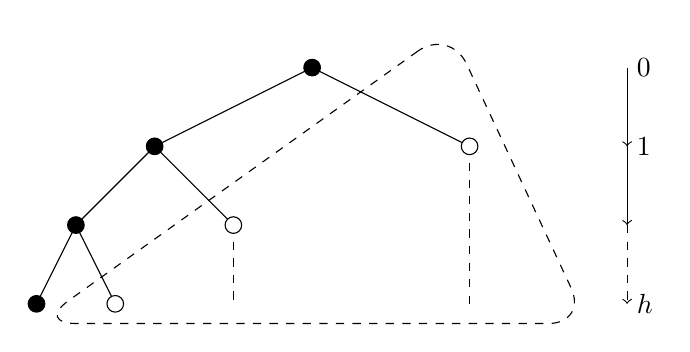
\begin{tikzpicture}

    % Conexiones
    \draw (0,0) -- (-2,-1);
    \draw (0,0) -- (2,-1);

    \draw (-2,-1) -- (-3,-2);
    \draw (-2,-1) -- (-1,-2);

    \draw (-3,-2) -- (-3.5,-3);
    \draw (-3,-2) -- (-2.5,-3);

    \draw[dashed] (2,-1) -- (2,-3);
    \draw[dashed] (-1,-2) -- (-1,-3);


    % Puntos
    \filldraw (0,0) circle [radius=3pt, fill=black];

    \filldraw (-2,-1) circle [radius=3pt, fill=black];
    \filldraw[draw=black, fill=white] (2,-1) circle [radius=3pt];

    \filldraw (-3,-2) circle [radius=3pt, fill=black];
    \filldraw[draw=black, fill=white] (-1,-2) circle [radius=3pt];

    \filldraw (-3.5,-3) circle [radius=3pt, fill=black];
    \filldraw[draw=black, fill=white] (-2.5,-3) circle [radius=3pt];

    % Niveles
    \draw[->] (4,0) -- (4,-1);
    \node[anchor=west] at (4,0) {0};

    \draw[->] (4,-1) -- (4,-2);
    \node[anchor=west] at (4,-1) {1};


    \draw[dashed, ->] (4,-2) -- (4,-3);
    \node[anchor=west] at (4,-3) {$h$};

    % Envoltorio

    \draw[dashed] [rounded corners=0.5cm] (1.75,0.5) -- (-3.5,-3.25)[rounded corners=0.5cm] -- (3.5,-3.25) -- cycle;


\end{tikzpicture}